\section{TP 9}


\subsection*{Exercice 1}
Soient $x, y$ et $z$ trois n\oe{}uds distincts. On dit que $x$ est un \emph{n\oe{}ud pivot} pour $y$ et $z$ si tous les chemins les plus courts entre $y$ et $z$ passent par $x$.

\begin{enumerate}
\item Donnez un exemple d'un graphe o\`{u} tous les n\oe{}uds sont un n\oe{}ud pivot pour au moins une paire de n\oe{}uds.
\item Donnez un exemple d'un graphe o\`{u} tous les n\oe{}uds sont un n\oe{}ud pivot pour au moins trois paires de n\oe{}uds.
\item Soit $G$ un graphe qui repr\'{e}sente les liens d'amiti\'{e} d'un groupe de personnes. Si on suppose que la probabilit\'{e}e que deux personnes qui ne sont pas amies au
temps $t$ deviennent amies au temps $t + 1$ est inversement proportionelle a la distance entre elles, quel est l'effet sur la probabilit\'{e} de retirer un personne pivot du graphe?
\item Montrez qui si tous les n\oe{}uds sont un n\oe{}ud pivot pour au moins une paire de n\oe{}uds alors le graphe poss\'{e}de au moins un cycle.
\end{enumerate}

\subsubsection*{Solution}

\begin{enumerate}
	\item On prend $G = $
\begin{center}
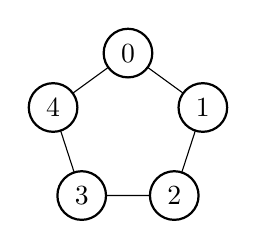
\begin{tikzpicture}
\tikzstyle{node}=[circle,draw,thick,fill=white]
\draw (90:1) node[node]{0}
-- (162:1) node[node]{4}
-- (234:1) node[node]{3}
-- (306:1) node[node]{2}
-- (378:1) node[node]{1}
-- cycle;
\end{tikzpicture}
\end{center}
$\forall i$ le noeud $i$ est pivot de $(i-1)\&(i+1)$ (modulo 5).

	\item On prend $G = $
\begin{center}
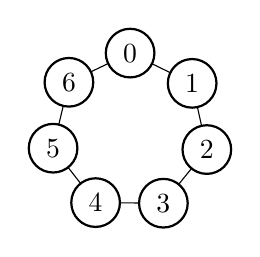
\begin{tikzpicture}
\tikzstyle{node}=[circle,draw,thick,fill=white]
\draw (90:1) node[node]{0}
-- (141:1) node[node]{6}
-- (192:1) node[node]{5}
-- (244:1) node[node]{4}
-- (295:1) node[node]{3}
-- (347:1) node[node]{2}
-- (398:1) node[node]{1}
-- cycle;
\end{tikzpicture}
\end{center}

$\forall i$ le noeud $i$ est pivot de :
$(i-1) \& (i+1)$, $(i-1) \& (i+2)$ et $(i-2) \& (i+1)$
(modulo 7).
	\item Retirer le noeud pivot augmente la distance entre 2 personnes. Donc la probabilité que celles ci deviennent amies au temps $t+1$ diminue.

	\item On prouve d'abord que si un graphe n'a pas de cycle alors il possède au moins un noeud de degré 1.

Supposons que $G$ n'a pas de cycle et $V$ l'ensemble fini de ses noeuds.
Soit $x \in V$. On construit une séquence $P = (x_1, x_2, x_3, ...)$. Pour choisir $x_i (i>1)$, on prend un voisin de $x_{i-1}$ qiu n'a pas encore été choisi. Comme $V$ est fini, ce processus doit finir et on obtient $P= (x_1, x_2, x_3,...,x_k)$.
Le noeud $k$ a un degré 1 car sinon il a un voisin $y\neq x_{k-1}$. Si $y \in P$ : Contradiction.
Si $y \notin P$, $x_k$ n'est pas la fin de la séquance : Contradiction.

On prouve ensuite que un noeud de degré un ne peu pas etre pivot.

Soit $x\in V$ tel que deg$(x)=1$.
Par hypothèse $x$ est pivot d'une paire $(y,z)$.
Donc il existe un chemin le plus court entre $y$ et $z$ qui passe bien par $x$.
Soit $w$ le seul voisin de $x$.
Mais alors il existe un chemin encore plus court : $(y, ..., w,...,z)$ qui ne passe pas par $x$.

% Insérer graphe

\end{enumerate}
\subsection*{Exercice 2}
Soient $x, y$ et $z$ trois n\oe{}uds distincts. On dit que $x$ est un \emph{gardien} de $y$ et $z$ si tous les chemins entre $y$ et $z$ passent par $x$.
On dit qu'un n\oe{}ud $x$ est un \emph{gardien locale} s'il existent deux voisins de $x$ qui ne sont pas connect\'{e}s directement.

\begin{enumerate}
\item Donnez un exemple d'un graphe o\`{u} au moins la moiti\'{e} des n\oe{}uds sont
gardiens.
\item Donnez un exemple d'un graphe o\`{u} il n'y a pas de gardiens mais chaque n\oe{}ud est un gardien locale.
\item Quel est l'impacte sur un graphe de retirer un gardien?
\end{enumerate}

\subsubsection*{Solution}
\begin{enumerate}
	\item Les noeuds 1 et 2 sont gardien entre 0 et 3

\begin{center}
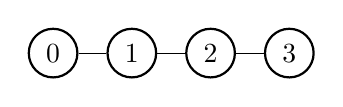
\begin{tikzpicture}
    \tikzstyle{node}=[circle,draw,thick,fill=white]
    \node[node] (0) at (0,0) {0};
    \node[node] (1) at (1,0) {1};
    \node[node] (2) at (2,0) {2};
    \node[node] (3) at (3,0) {3};

    \draw (0) -- (1);
    \draw (1) -- (2);
    \draw (2) -- (3);
\end{tikzpicture}
\end{center}

	\item  \hspace{1em}
	\vspace{1em}

\begin{center}
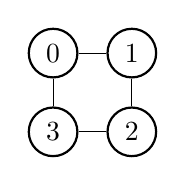
\begin{tikzpicture}
\tikzstyle{node}=[circle,draw,thick,fill=white]
    \node[node] (0) at (0,0) {0};
    \node[node] (1) at (1,0) {1};
    \node[node] (2) at (1,-1) {2};
    \node[node] (3) at (0,-1) {3};

    \draw (0) -- (1);
    \draw (1) -- (2);
    \draw (2) -- (3);
    \draw (3) -- (0);
\end{tikzpicture}
\end{center}

	\item Le graphe n'est plus connexe
\end{enumerate}

\subsection*{Exercice 3}

\begin{enumerate}
 \item Comment peut-on faire pour calculer efficacement les distances d'un n\oe{}uds a tout les autres?
 \item Un graphe est biparti si on peut s\'{e}parer les n\oe{}uds en deux ensembles $V_1$ et $V_2$ tells que
 $V_1 \cap V_2 = \emptyset$, $V_1 \cup V_2 = V$ et il n'y a pas d'ar\^{e}tes entre aucune paire de n\oe{}uds de $V_1$ et
 pas d'ar\^{e}tes entre aucune paire de n\oe{}uds de $V_2$. Soit $G$ un graphe connexe et $d_0(x)$ la distance du n\oe{}ud
 $0$ au n\oe{}ud $x$. Comment peut-on v\'{e}rifier que $G$ est bipartit a partir de $d_0$?
\end{enumerate}

\subsubsection*{Solution}
\begin{enumerate}

	\item On utilise l'algorithme BFS qui utilise une \texttt{Queue FIFO}
\begin{enumerate}
    \item Mettre le n\oe{}ud dans la Queue.
    \item Retirer le n\oe{}ud du début de la Queue pour l'examiner.
    \item Mettre tous les voisins non explorés dans la Queue.
    \item Si la file n'est pas vide reprendre à l'étape 2.
\end{enumerate}

Exemple :

\begin{tabular}{lll}
    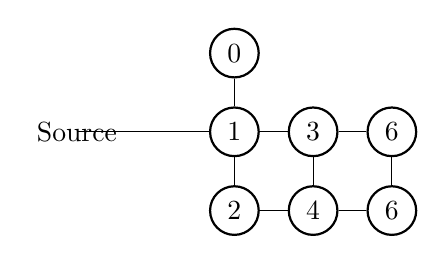
\begin{tikzpicture}
    \tikzstyle{node}=[circle,draw,thick,fill=white]
    \node[node] (2) at (0,0) {2};
    \node[node] (1) at (0,1) {1};
    \node[node] (0) at (0,2) {0};
    \node[node] (4) at (1,0) {4};
    \node[node] (3) at (1,1) {3};
    \node[node] (5) at (2,1) {6};
    \node[node] (6) at (2,0) {6};
    \node[] (S) at (-2,1) {Source};

    \draw (S) |- (1.west);
    \draw (0) -- (1);
    \draw (1) -- (2);
    \draw (3) -- (1);
    \draw (2) -- (4);
    \draw (4) -- (3);
    \draw (3) -- (5);
    \draw (6) -- (4);
    \draw (5) -- (6);
\end{tikzpicture}
&

&
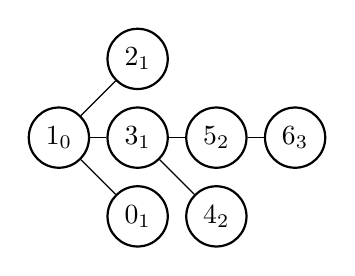
\begin{tikzpicture}
    \tikzstyle{node}=[circle,draw,thick,fill=white]
    \node[node] (1) at (0,1) {$1_{0}$};
    \node[node] (0) at (1,0) {$0_{1}$};
    \node[node] (3) at (1,1) {$3_{1}$};
    \node[node] (2) at (1,2) {$2_{1}$};
    \node[node] (5) at (2,1) {$5_{2}$};
    \node[node] (4) at (2,0) {$4_{2}$};
    \node[node] (6) at (3,1) {$6_{3}$};

    \draw (1) -- (0);
    \draw (1) -- (3);
    \draw (1) -- (2);
    \draw (3) -- (5);
    \draw (3) -- (4);
    \draw (5) -- (6);
\end{tikzpicture}
\end{tabular}

\item On vérifie qu'il n'existe pas d'arètes $(x,y)$ tel que $d_0(x)$ et $d_0(y)$ ont la meme parité

\end{enumerate}

% \vspace{0.5cm}
%
% \subsection*{Exercice }
% Soient $x, y$ et $z$ trois n\oe{}uds distincts. On dit que $x$ est un \emph{gardien} de $y$ et $z$ si tous les chemins entre $y$ et $z$ passent par $x$.
% On dit qu'un n\oe{}ud $x$ est un \emph{gardien locale} s'il existent deux voisins de $x$ qui ne sont pas connect\'{e}s directement.
%
% \begin{enumerate}
% \item Donnez un exemple d'un graphe o\`{u} au moins la moiti\'{e} des n\oe{}uds sont
% gardiens.
% \item Donnez un exemple d'un graphe o\`{u} il n'y a pas de gardiens mais chaque n\oe{}ud est un gardien locale.
% \end{enumerate}
%

\subsection*{Exercice 4}
Le \emph{diam\`{e}tre} d'un graphe connexe est la distance maximum entre toutes les paires de n\oe{}uds.
La \emph{distance moyenne} d'un graphe connexe c'est la moyenne des distances entre toutes les paires de n\oe{}uds. Formellement
$$
diam(G) = \max_{u, v} d(u, v)
$$
et
$$
l_G = \frac{1}{V (V - 1)} \sum_{u \neq v} d(u, v)
$$
o\'{u} $V$ est le nombre de n\oe{}uds de $G$.
\begin{enumerate}
\item Calculez le diam\`{e}tre et la distance moyenne du graphe $G_n$ suivant:
\begin{center}
\begin{tikzpicture}
\node[draw, circle] (A) at (0, 0) {0};
\node[draw, circle] (B) at (2, 0) {1};
\node[draw, circle] (C) at (4, 0) {2};
\node[draw, circle] (D) at (6, 0) {3};
\draw (A) -- (B) -- (C) -- (D);
\draw[dashed] (7, 0) circle (2);
\node at (9.5, 1) {$K_n$};
\draw (D) -- (7, 1);
\node at (7, 0.4) {$\vdots$};
\draw (D) -- (7, -0.5);
\draw (D) -- (7, -1);
\end{tikzpicture}
\end{center}
o\`{u} $K_n$ est le graphe complet avec $n$ n\oe{}uds. Par example, $G_4$ est le graphe:
\begin{center}
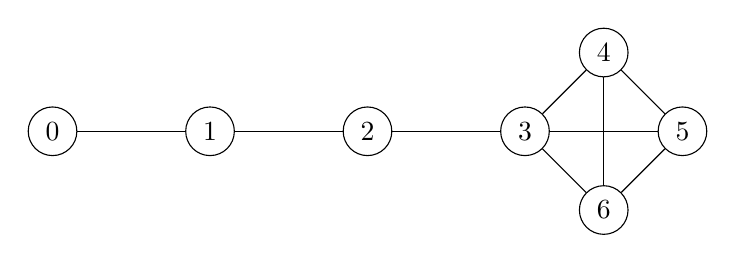
\begin{tikzpicture}
\node[draw, circle] (A) at (0, 0) {0};
\node[draw, circle] (B) at (2, 0) {1};
\node[draw, circle] (C) at (4, 0) {2};
\node[draw, circle] (D) at (6, 0) {3};
\node[draw, circle] (E) at (7, 1) {4};
\node[draw, circle] (F) at (8, 0) {5};
\node[draw, circle] (G) at (7, -1) {6};

\draw (A) -- (B) -- (C) -- (D);
\draw (D) -- (E);
\draw (D) -- (F);
\draw (D) -- (G);
\draw (E) -- (F);
\draw (E) -- (G);
\draw (G) -- (F);
\end{tikzpicture}
\end{center}


\item Montrez qu'il existe un graphe $G$ avec plus de $7$ n\oe{}uds tel que
$$\frac{diam(G)}{l_G} = 2$$

\end{enumerate}


% \subsection*{Exercice }
% Calculez le coefficient regroupement de A et de B dans le graphe suivant:
% \begin{center}
% \begin{tikzpicture}
% \node[draw, circle] (A) at (0, 0)   {A};
% \node[draw, circle] (B) at (-2, 1)  {B};
% \node[draw, circle] (C) at (2, 1)   {C};
% \node[draw, circle] (D) at (2, -1)  {D};
% \node[draw, circle] (E) at (-2, -1) {E};
% \node[draw, circle] (F) at (-4, 0)  {F};
% \draw (A) -- (B);
% \draw (A) -- (C) -- (D);
% \draw (A) -- (D);
% \draw (A) -- (E) -- (B);
% \draw (B) -- (F) -- (E);
% \end{tikzpicture}
% \end{center}
%
%
% \vspace{0.5cm}

\subsubsection*{Solution}
\begin{enumerate}

	\item dim$(G) = 4$

Selon la table des distance:

\begin{tabular}{c|ccccc}
    &0&1&2&3& >3 \\
    \hline
    0 & 0& 1& 2& 3& 4\\
    1 & 1& 0&1& 2& 3\\
    2 & 2& 1& 0& 1&2\\
    3 & 1& 2& 3& 0&1\\
    >3 & 4& 3& 2& 1& 1 (0 si lui meme)\\
\end{tabular}

On peut calculer $\sum_{u\neq v} d(u,v)$.

\begin{align*}
    \sum_{u\neq v} d(u,v) =& 6 + 4(n-1)\\
    &+ 4 + 3(n-1)\\
    &+4+2(n-1)\\
    &+6+(n-1)\\
    &+(n-1)(10 + (n-2))\\
    =& 20 + (n-1)(4+3+2+1) + (n-1)(9 + (n-2))\\
    =& 20 + 10(n-1) + 9(n-1) + (n-1)^2\\
    =& 20 + 19(n-1) + (n-1)^2\\
    & \Rightarrow l_G (n) = \dfrac{n^2 + 17n + 2}{n^2 + 5n + 6}
\end{align*}


	\item $\dfrac{\text{diam}(G)}{l_G} = \dfrac{4}{l_G} =2$
\begin{align*}
    & \dfrac{4n^2 + 20n + 24}{n^2 + 17n + 2} = 2\\
    & \Rightarrow 4n^2 + 20n + 24 = 2n^2 + 34n + 4\\
    & \Rightarrow 2n^2 - 14n + 2\\
    & \Rightarrow n = 5\hspace{1em}\&\hspace{1em} n = 2\\
\end{align*}

Or $G$ doit comporter au moins 7 noeuds donc $G(5)$.

\end{enumerate}

\subsection*{Exercice 5}
On suppose qu'on est dans une communaut\'{e} ou les amiti\'{e}s sont repr\'{e}sent\'{e}es par un graphe $G$ connexe avec $n$ n\oe{}uds.
Si chaque jour les amis des amis se rencontrent et deviennent amis, on s'interesse au nombre de jours $T(G)$ n\'{e}cessaires
pour que tout le monde deviennent ami, c'est-\`{a}-dire, pour le graphe deviennent $K_n$ (un graphe complet).
\begin{enumerate}
\item Supposons que $G = P_n$ (le chemin avec $n$ n\oe{}uds) et $T(P_n)$.
\item M\^{e}me question pour $G = C_n$ (le cycle avec $n$ n\oe{}uds).
\item Quel est la valeur de $T(G)$ en g\'{e}neral?
\end{enumerate}

\subsubsection*{Solution}
\begin{enumerate}

	\item Soit $A(i)$, les amis de $0$ au jour $i$.
\begin{align*}
    A(0) =& \{1 \} \\
    A(1) =& \{1,2 \}\\
    A(2) =& \{1,2,3,4 \}\\
    A(3) =& \{1,2,3,4,5,6,7,8, \}\\
    A(i) =& \{x+y | x,y \in A(i-1) \} \\
         =& \{1,2,3,..., 2^i \} \\
    T(P_n) =& \lceil \log_2 (n) \rceil
\end{align*}


	\item Le noeud le plus loin de $0$ dans un cycle de $n$ noeuds, est le noeud $\left\lfloor \dfrac{n}{2} \right\rfloor$
$$ T(C_n) = \left\lceil \log_2 \left(\left\lfloor \dfrac{n}{2} \right\rfloor \right) \right\rceil $$

	\item En général les noeuds à distance maximum prennent le plus de temps. Cette distance est le diamètre du graphe. Donc :
$$ T(G) = \left\lceil \log_2 \left( \text{dim}(G) \right) \right\rceil $$


\end{enumerate}
%
% \subsection*{Exercice }
% Calculez le coefficient de regroupement d'un n\oe{}ud de $C_n$, o\`{u} $n \geq 3$. Calculez le coefficient de regroupement de ce n\oe{}ud ap\`{e}s avoir ajout\'{e} les ar\^{e}tes entre les amis des amis dans le graphe. Commentez.
%
%
%
% \subsection*{Exercice }
% \'{E}noncez la propri\'{e}t\'{e} de fermeture triadique forte. Est-ce que le graphe suivant poss\`{e}de cette propri\'{e}t\'{e}?
%
% \begin{center}
% \begin{tikzpicture}
% \node[draw, circle] (A) at (0, 0) {A};
% \node[draw, circle] (B) at (2, 0) {B};
% \node[draw, circle] (C) at (0, -2) {C};
% \node[draw, circle] (D) at (-2, 0) {D};
% \node[draw, circle] (E) at (0, -4) {E};
% \node[draw, circle] (F) at (2, -2) {F};
% \node[draw, circle] (G) at (-2, -4) {G};
% \draw (G) -- (D) -- (A) -- (C) -- (F);
% \draw (C) -- (E);
% \draw[dashed] (G) -- (A) -- (B) -- (F) -- (E) -- (G);
% \draw[dashed] (D) -- (C);
%
% \draw (4, -1) -- (5, -1) node[anchor = west] {lien fort};
% \draw[dashed] (4, -2) -- (5, -2) node[anchor = west] {lien faible};
% \end{tikzpicture}
% \end{center}
%
% Supposons qu'un graphe poss\`{e}de la propri\'{e}t\'{e} de fermeture triadique forte. Si un lien faible devient fort, est-ce que cette propri\'{e}t\'{e} se maintien toujours? Et si un lien fort devient faible?
%
%
